\section{Classifier-Free Guidance (CFG)}
\begin{frame}{}
    \LARGE Classifier-Free Guidance (CFG)
\end{frame}

\begin{frame}{What is Classifier-Free Guidance?}
    \begin{itemize}
        \item A technique to improve the quality of text-to-image generation by controlling the influence of text prompts.
        \item It allows for generating images that are more aligned with the provided text while maintaining diversity.
        \item CFG is particularly useful in diffusion models, enhancing the coherence between text and generated images.
    \end{itemize}
\end{frame}

\begin{frame}[allowframebreaks]{Key Properties of Classifier-Free Guidance}
    \begin{itemize}
        \item \textbf{Balances realism and fidelity:} Adjusts the trade-off between generating realistic images and staying faithful to the text prompt.
        \item \textbf{No external classifier needed:} Removes the requirement for a separate classifier to guide the generation process.
        \item \textbf{Score interpolation:} Interpolates between conditional (with prompt) and unconditional (without prompt) model outputs to control guidance strength.
    \end{itemize}
\framebreak

    \begin{figure}
        \centering
        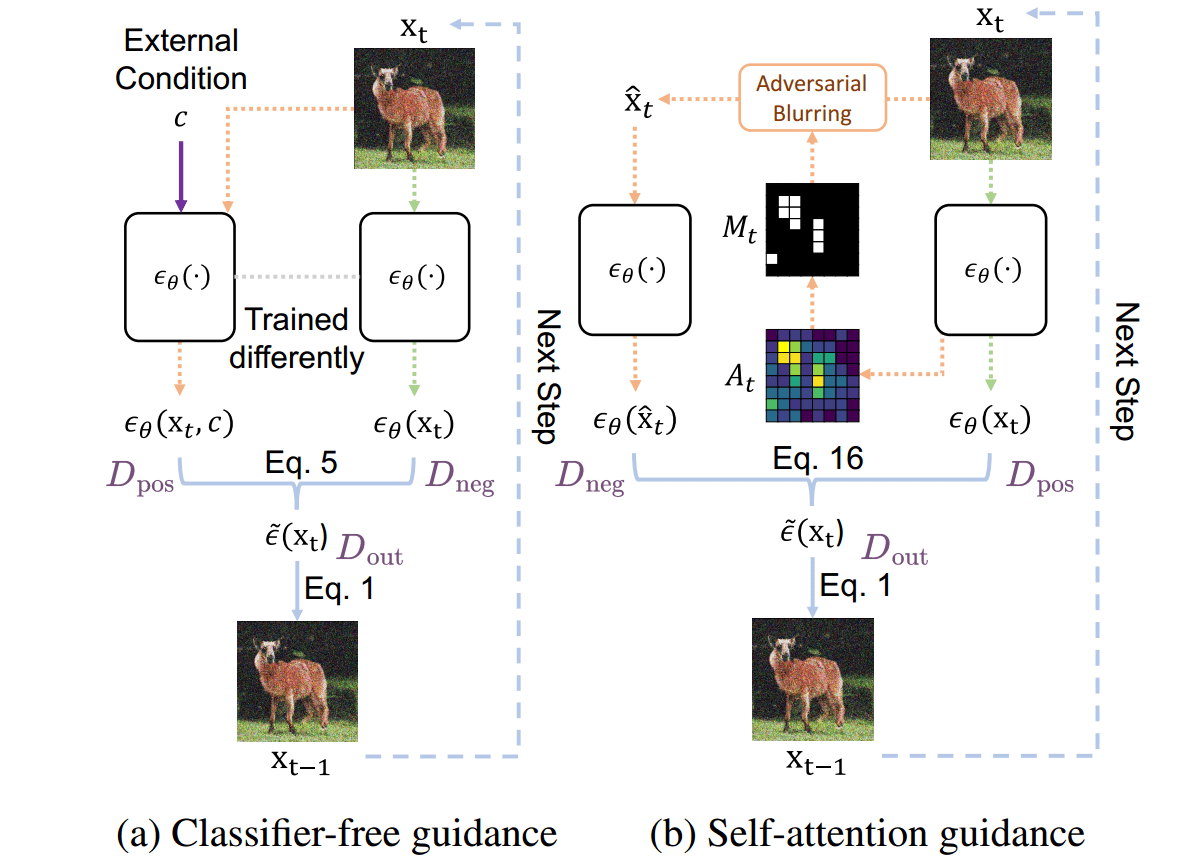
\includegraphics[width=\linewidth,height=0.8\textheight,keepaspectratio]{images/vision+text/classifier-free-guidance.png}
        \caption*{Illustration of Classifier-Free Guidance in text-to-image generation.}
    \end{figure}

\framebreak

    \textbf{How does it work?}
    \begin{itemize}
        \item The model generates images based on both the text prompt and random noise.
        \item By adjusting the guidance scale, users can control how much the text influences the final image.
        \item Higher guidance scales lead to images that are more closely aligned with the text, while lower scales allow for more creative freedom.
    \end{itemize}
\framebreak

    \begin{figure}
        \centering
        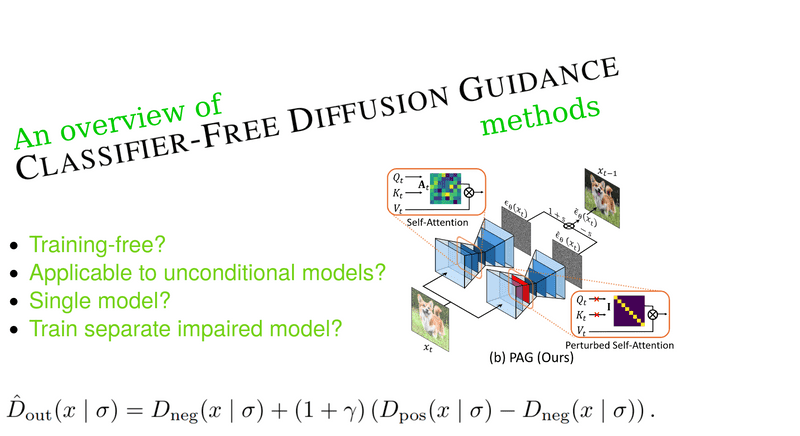
\includegraphics[width=\linewidth,height=0.8\textheight,keepaspectratio]{images/vision+text/classifier-free-guidance-2.png}
        \caption*{Illustration of Classifier-Free Guidance in text-to-image generation.}
    \end{figure}
\end{frame}


\begin{frame}[fragile]{Implementation of Classifier-Free Guidance}
    \begin{itemize}
        \item \textbf{Duplicate forward pass:} For each input, perform two forward passes through the model:
        \begin{itemize}
            \item One with the conditioning (e.g., text prompt)
            \item One without conditioning (unconditional)
        \end{itemize}
        \item \textbf{Combine outputs:} The final score is computed as:
        \[
            s = s_{\text{uncond}} + w \cdot (s_{\text{cond}} - s_{\text{uncond}})
        \]
        where:
        \begin{itemize}
            \item $s_{\text{cond}}$ is the model output with conditioning
            \item $s_{\text{uncond}}$ is the model output without conditioning
            \item $w$ is the guidance scale parameter
        \end{itemize}
        \item \textbf{Effect of $w$:} Controls the strength of guidance. Higher $w$ enforces stronger adherence to the prompt.
    \end{itemize}
\end{frame}

\begin{frame}{Benefits of Classifier-Free Guidance}
    \begin{itemize}
        \item \textbf{Simpler and faster:} Eliminates the need for a separate classifier, reducing complexity and computational overhead.
        \item \textbf{Effective for text-guided diffusion:} Provides strong alignment between generated images and text prompts in diffusion models.
        \item \textbf{Foundation of modern T2I systems:} Forms the basis of Stable Diffusion XL (SDXL) and other state-of-the-art text-to-image generation systems.
    \end{itemize}
\end{frame}